\begin{equation}
    \begin{gathered}
        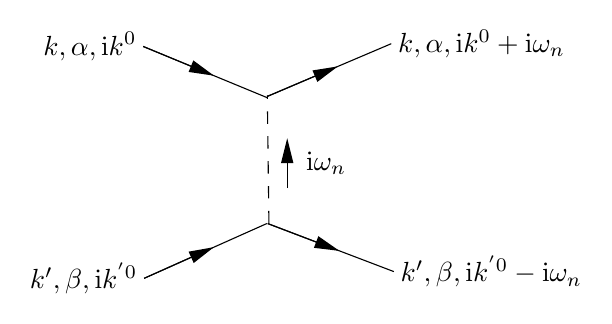
\begin{tikzpicture}[x=0.75pt,y=0.75pt,yscale=-1,xscale=1]
            %uncomment if require: \path (0,300); %set diagram left start at 0, and has height of 300
            
            %Straight Lines [id:da8811257678790001] 
            \draw    (120.17,192.51) -- (151.95,178.32) ;
            \draw [shift={(153.77,177.5)}, rotate = 515.9300000000001] [fill={rgb, 255:red, 0; green, 0; blue, 0 }  ][line width=0.08]  [draw opacity=0] (12,-3) -- (0,0) -- (12,3) -- cycle    ;
            %Straight Lines [id:da09245372313993339] 
            \draw    (120.17,192.51) -- (179.26,166.12) ;
            
            %Straight Lines [id:da5212176663602186] 
            \draw  [dash pattern={on 4.5pt off 4.5pt}]  (180.29,166.04) -- (179.51,104.35) ;
            %Straight Lines [id:da3600618743982982] 
            \draw    (179.7,166.12) -- (212.38,178.57) ;
            \draw [shift={(214.25,179.28)}, rotate = 200.85] [fill={rgb, 255:red, 0; green, 0; blue, 0 }  ][line width=0.08]  [draw opacity=0] (12,-3) -- (0,0) -- (12,3) -- cycle    ;
            %Straight Lines [id:da4597439893236821] 
            \draw    (179.7,166.12) -- (240.46,189.26) ;
            
            %Straight Lines [id:da6718339117636689] 
            \draw    (119.72,80.8) -- (151.97,94.12) ;
            \draw [shift={(153.82,94.88)}, rotate = 202.44] [fill={rgb, 255:red, 0; green, 0; blue, 0 }  ][line width=0.08]  [draw opacity=0] (12,-3) -- (0,0) -- (12,3) -- cycle    ;
            %Straight Lines [id:da24771739237802826] 
            \draw    (119.72,80.8) -- (179.69,105.57) ;
            
            %Straight Lines [id:da9719269379719568] 
            \draw    (179.57,104.84) -- (211.65,91.2) ;
            \draw [shift={(213.49,90.41)}, rotate = 516.96] [fill={rgb, 255:red, 0; green, 0; blue, 0 }  ][line width=0.08]  [draw opacity=0] (12,-3) -- (0,0) -- (12,3) -- cycle    ;
            %Straight Lines [id:da6203152798089022] 
            \draw    (179.57,104.84) -- (239.22,79.47) ;
            
            %Straight Lines [id:da7749523816411303] 
            \draw    (189.09,149.1) -- (189.09,127.04) ;
            \draw [shift={(189.09,125.04)}, rotate = 450] [fill={rgb, 255:red, 0; green, 0; blue, 0 }  ][line width=0.08]  [draw opacity=0] (12,-3) -- (0,0) -- (12,3) -- cycle    ;
            
            % Text Node
            \draw (117.72,80.8) node [anchor=east] [inner sep=0.75pt]    {$\boldsymbol{k} ,\alpha ,\mathrm{i} k^{0}$};
            % Text Node
            \draw (241.22,79.47) node [anchor=west] [inner sep=0.75pt]    {$\boldsymbol{k} ,\alpha ,\mathrm{i} k^{0} +\mathrm{i} \omega _{n}$};
            % Text Node
            \draw (118.17,192.51) node [anchor=east] [inner sep=0.75pt]    {$\boldsymbol{k} ',\beta ,\mathrm{i} k^{'0}$};
            % Text Node
            \draw (242.46,189.26) node [anchor=west] [inner sep=0.75pt]    {$\boldsymbol{k} ',\beta ,\mathrm{i} k^{'0} -\mathrm{i} \omega _{n}$};
            % Text Node
            \draw (197,130.4) node [anchor=north west][inner sep=0.75pt]    {$\mathrm{i} \omega _{n}$};
            \end{tikzpicture}
    \end{gathered} = - f_{\alpha \beta \vb*{k} \vb*{k}'},
    \label{eq:fermi-liquid-vertex}
\end{equation}